

În urma rulării a tuturor fișierelor atât pentru alpha\_beta\_CROWN, cât și pentru NeuralSAT am obținut un număr de instanțe, pentru care timpul alocat verificării a fost depășit, egal cu 0. Prin urmare nu avem penalități pentru niciunul dintre tool-uri.

Totodată am obținut un Total verified egal cu 8, și un Total falsified egal cu 11 pentru ambele tool-uri. Pentru alpha\_beta\_CROWN rezultatele sunt identice cu cele din competiție. În cazul NeuralSAT, se poate observa că solver-ul
a suferit îmbunătățiri în urma livrărilor constante făcute de dezvoltatori deoarece rezultatele obținute de noi au strâns un scor perfect de 100\%, mult peste cel obținut de solver în cadrul competiției.

\begin{table}[h]
\centering
\begin{tabular}{clcccccc}
\hline
\# & Tool & Verified & Falsified & Fastest & Penalty & Score & Percent \\ \hline
1 & \(\alpha\)-\(\beta\) CROWN & 8 & 11 & 0 & 0 & 190 & 100\% \\
2 & NeuralSAT & 8 & 11 & 0 & 0 & 190 & 100\% \\ \hline
\end{tabular}
\end{table}

Din tabelul de mai jos putem sa ne dam seama(mai mult sau mai puțin) că formula de calculare a scorului este: 

\[
\mathbf{\rightarrow \textbf{Verified} \times 10 + \textbf{Falsified} \times 10 - \textbf{Penalty} \times 150}
\]


Procentajul reprezintă scorul obținut exprimat ca procent din scorul maxim
posibil, oferind o imagine de ansamblu asupra performanței, iar formula de calcul
este:
\[
\mathbf{\frac{\textbf{Score} \times 100}{\textbf{max}(\textbf{Score})}}
\]

\begin{figure}[h]
\centering 
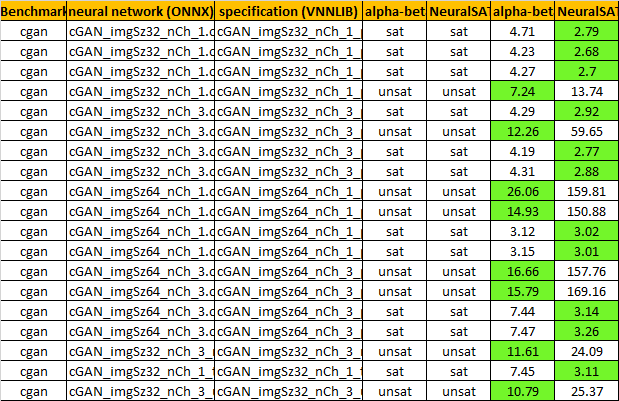
\includegraphics[width=0.8\linewidth]{imagini/interpretare rezultate/alpha-beta-CROWN_vs_NeuralSAT.png}
\caption{Comparare rezultate NeuralSAT vs alpha-beta-CROWN}
\label{fig:image2} 
\end{figure}
\
Analizând datele din tabelul de mai sus, putem observa că în cazul instanțelor cu rezultat satisfiabil (sat) verificatorul NeuralSAT a obținut timpi puțîn mai reduși de execuție decât alpha-beta-CROWN. Pe de altă parte, în cazul instanțelor cu rezultat nesatisfiabil (unsat) timpii de execuție obținuți de alpha-beta-CROWN sunt semnificativ mai reduși decât cei obținuți de NeuralSAT. Acest lucru este evidențiat și in graficul prezentat mai jos, graficul arată distribuirea timpilor de execuție pentru ambele tool-uri, comparând instanța cu instanța.



\begin{figure}[h]
\centering 
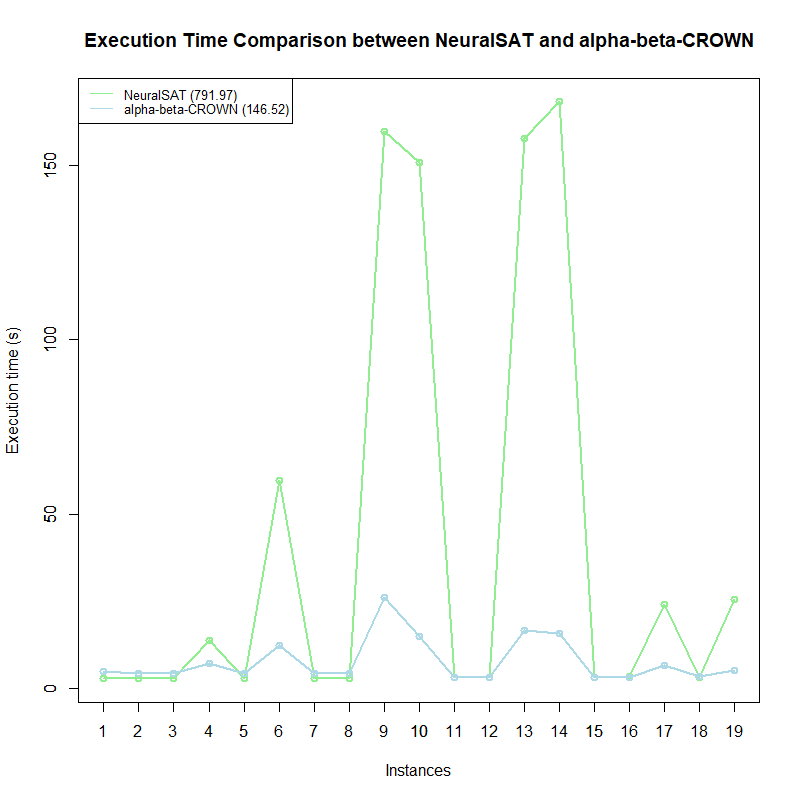
\includegraphics[width=0.8\linewidth]{imagini/interpretare rezultate/Exec_time_comparison.png}
\caption{Comparare rezultate NeuralSAT vs alpha-beta-CROWN}
\label{fig:image2} 
\end{figure}
\
Cel de al doilea grafic prezintă suma timpilor de execuție pe parcursul rulării tuturor celor 19 instanțe pe ambele verificatoare. Din acest grafic se poate trage concluzia că alpha-beta-CROWN este un tool mult mai eficient din punct de vedere a timpului de execuție.

\begin{figure}[h]
\centering 
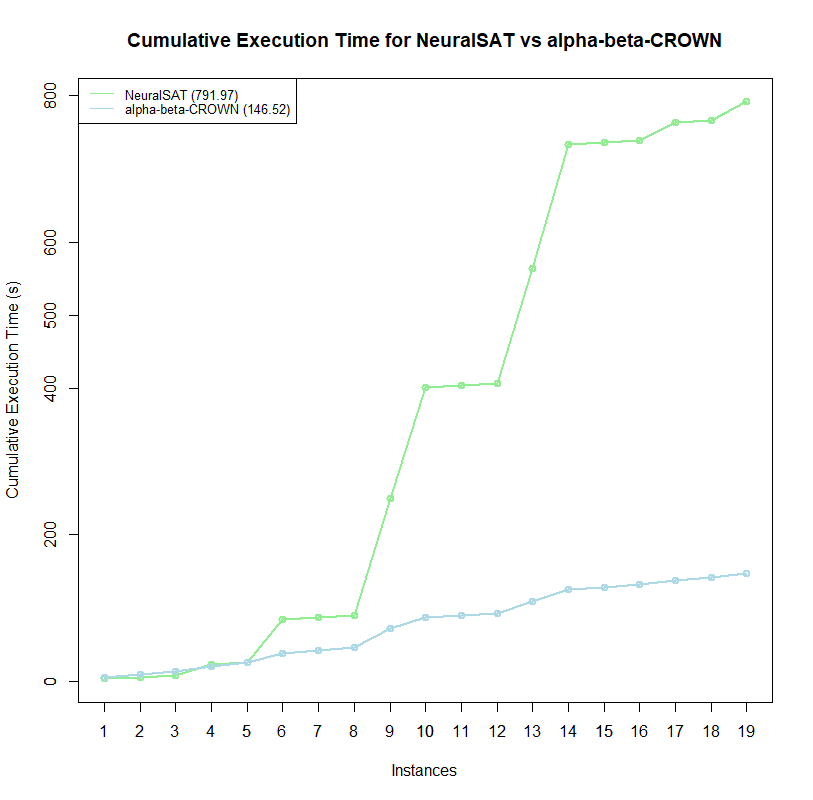
\includegraphics[width=0.8\linewidth]{imagini/interpretare rezultate/cumulative_NeuralSAT_vs_abC.png}
\caption{}
\label{fig:image2} 
\end{figure}
\



